\section{Exploratory data analysis}
\label{sec:eda}

\subsection{Data description}

\BL{T}he dataset used in this study was extracted from the project MonitorAr-Rio
\cite{dataset-rio-ar-quality}. The table contains hourly data observations, separated by
pollutant, weather condition, and monitoring stations' characteristics from
the city of Rio de Janeiro. Table
\ref{tab:measured-data} informs the most important variables used, and Table
\ref{tab:pollutants-measured} indicates the measured pollutants per monitoring
station. The events start on January 1,
2011,
and end on March 31, 2021, totalizing 661,662 records.

The missing values (Table \ref{tab:missing-values}) for each of the main variables used in this work 
are around 10\%. Some meteorological variables have more than 10\% of missing values, which is a lot.
The CO gas has more missing values than the other gases because Pedra de
Guaratiba does not measure it. When this kind of absent value is disregarded,
CO has around 6\%. Imputation methods in Section \ref{sec:data-preprocessing}.

Almost 91\% of the values in the {\tt Chuva} column and 26\% of the {\tt RS} column are zero. If we consider the accumulated monthly amount of
rain, it seems to make sense, and it is comparable to other sources. 

We did not observe any pattern of missing values per year or monitoring
station. In 2012, over half of the wind information is missing, however other
features are stable. However, after 2016, UR dominates the number of absent
data. If we aggregate by time (hour, day, month, and year), and sum up the
values of the features of each station, there are less missing data,
proportionally, what. This
implies other stations can provide useful information. 

\begin{table*}[t]
    \centering
    \begin{tabular}{c|c|c|c|}
        \cline{2-4}
       & \textbf{Name} & \textbf{Type} & \textbf{Description}              \\ \hline
        \multicolumn{1}{|c|}{\multirow{7}{*}{\textbf{Meterological conditions}}} & Chuva         & float         & Rainfall (mm)                     \\ \cline{2-4} 
        \multicolumn{1}{|c|}{}                                                   & Pres          & float         & Atmospheric Pressure (mbar)       \\ \cline{2-4} 
        \multicolumn{1}{|c|}{}                                                   & RS            & float         & Solar radiation (w/m2)            \\ \cline{2-4} 
        \multicolumn{1}{|c|}{}                                                   & Temp          & float         & Temperature (°C)                  \\ \cline{2-4} 
        \multicolumn{1}{|c|}{}                                                   & UR            & float         & Relative humidity (\%)            \\ \cline{2-4} 
        \multicolumn{1}{|c|}{}                                                   & Dir\_Vento    & float         & Wind direction (°)                \\ \cline{2-4} 
        \multicolumn{1}{|c|}{}                                                   & Vel\_Vento    & float         & Wind speed (m/s)                  \\ \hline
        \multicolumn{1}{|c|}{\multirow{5}{*}{\textbf{Measurement conditions}}}   & Data          & datetime      & Measurement date and hour         \\ \cline{2-4} 
        \multicolumn{1}{|c|}{}                                                   & CodNum        & integer        & Number of the monitoring station  \\ \cline{2-4} 
        \multicolumn{1}{|c|}{}                                                   & Estação       & string        & Name of the monitoring station    \\ \cline{2-4} 
        \multicolumn{1}{|c|}{}                                                   & Lat           & float         & Latitude position of the station  \\ \cline{2-4} 
        \multicolumn{1}{|c|}{}                                                   & Lon           & float         & Longitude position of the station \\ \hline
        \end{tabular}
    \caption{Measured parameters by the program MonitorAr.}
    \label{tab:measured-data}
\end{table*}

\begin{table*}[t]
    \centering
    \begin{tabular}{|c|c|}
    \hline
    \textbf{Monitoring station}        & \textbf{Measured gases/particulates}              \\ \hline
    Centro (CA)             & O$_3$, CO, PM$_{10}$                              \\ \hline
    Copacabana (AV)         & SO$_2$, O$_3$, CO, PM$_{10}$                      \\ \hline
    São Cristóvão (SC)      & SO$_2$, O$_3$, CO, PM$_{10}$                      \\ \hline
    Tijuca (SP)             & SO$_2$, NOx, O$_3$, CO, PM$_{10}$                 \\ \hline
    Irajá (IR)              & SO$_2$, NOx, O$_3$, CO, HC, PM$_{2.5}$, PM$_{10}$ \\ \hline
    Bangu (BG)              & SO$_2$, NOx, O$_3$, CO, HC, PM$_{10}$             \\ \hline
    Campo Grande (CG)       & SO$_2$, NOx, O$_3$, CO, HC, PM$_{10}$             \\ \hline
    Pedra de Guaratiba (PG) & O$_3$, PM$_{10}$                                  \\ \hline
    \end{tabular}
    \caption{Pollutant data measured by each monitoring station. CO and HC are measured in (ppm), while the others are measured in (µg/m3).}
    \label{tab:pollutants-measured}
\end{table*}

\begin{figure*}[ht]
    \centering
    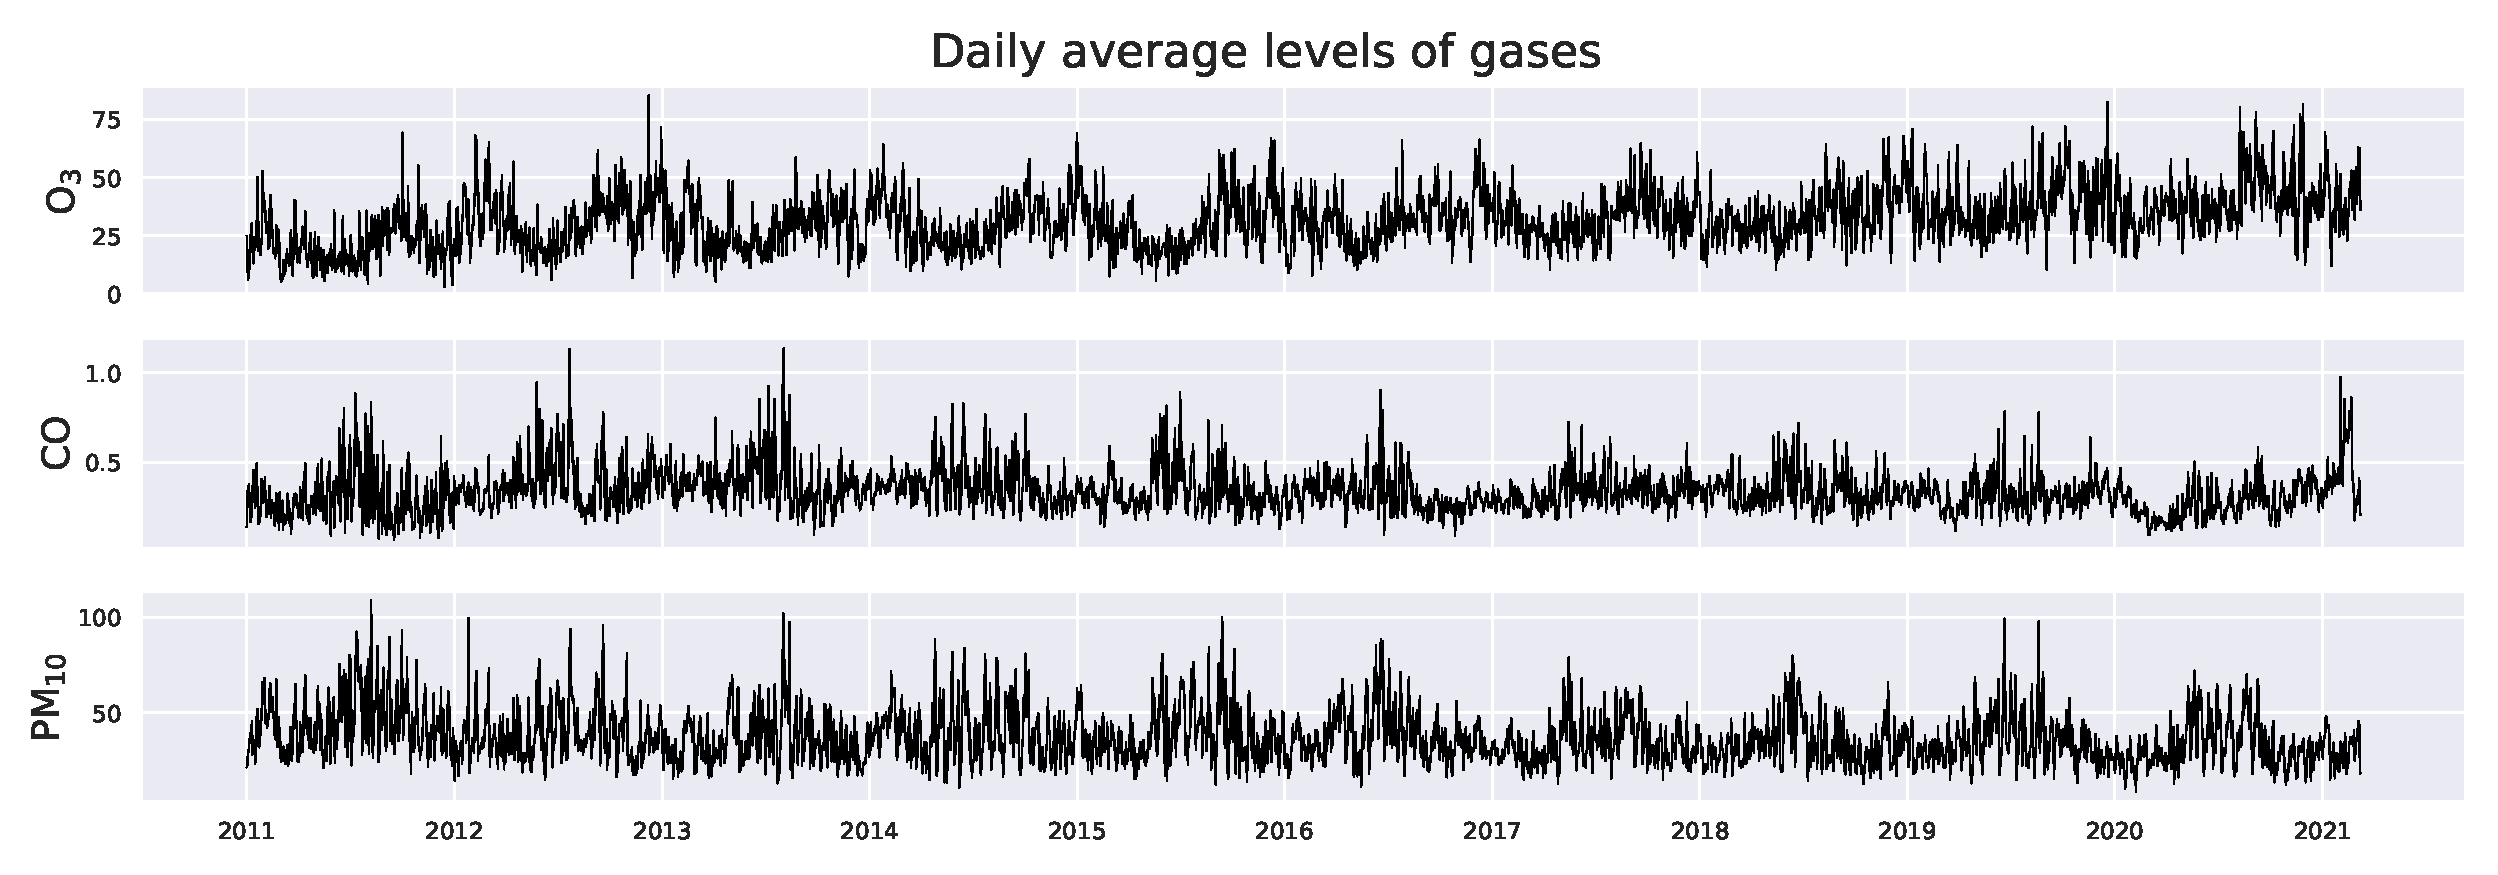
\includegraphics[width=\textwidth]{time-plots-gases.eps}
    \caption{Time series with diary average levels.}
    \label{fig:time-series-gases}
\end{figure*}

\begin{table}
    \centering
    \begin{tabular}{|c|c|}
        \hline
        {\bf Variable} & {\bf Missing values} \\\hline
        Chuva     &   15812 (2.38 \%) \\\hline
        Pres      &   15294 (2.31 \%) \\\hline
        RS        &   48260 (7.29 \%) \\\hline
        Temp      &   70617 (10.6 \%) \\\hline
        UR        &  110619 (16.7 \%) \\\hline
        Dir\_Vento &   90498 (13.6 \%) \\\hline
        Vel\_Vento &   90743 (13.7 \%) \\\hline
        CO        &  114179 (17.2 \%) \\\hline
        O3        &   37133 (5.61 \%) \\\hline
        PM10      &   36142 (5.46 \%) \\\hline
    \end{tabular}
    \caption{Missing data in absolute and proportional values of the main variables. Data, CodNum, Lat, and Lon do not have nan values.}
    \label{tab:missing-values}    
\end{table}

Table \ref{tab:statistics-variables} contains the summary statistics of the variables. The high skewness and kurtosis from {\tt
Chuva} column reaffirm the heavy tails of its distribution, or the presence of
outliers. The same occurs with {\tt Press}. This is interesting because, it is common to see days with
extreme values in meterological variables. In particular, the only hours with
precipitation greater than 100 mm were in May 2020 in Tijuca, what is
confirmed by weather references \cite{climatempo}. CO and PM$_{10}$ have high
kurtosis also and, therefore, can have outliers. 

\begin{table*}[t]
    \centering
    \begin{tabular}{|c|c|c|c|c|c|c|c|c|c|c|}
        \hline
        {} & {\bf Chuva} &  {\bf Pres} & {\bf RS} & {\bf Temp} & {\bf UR} &
        {\bf Dir} & {\bf Vel} & {\bf CO} & {\bf O3} & {\bf PM10} \\
        \hline
        {\bf Mean}  &       0.13 &    1014.65 &     152.82 &      26.12 &      70.90
        &     163.73 &       1.21 &       0.34 &      31.98 &      36.91 \\
        \hline
        {\bf Std}   &       1.64 &       5.68 &     244.37 &       4.90 &      18.35
        &      73.45 &       1.00 &       0.28 &      29.81 &      23.52 \\
        \hline
        {\bf Min}   &       0.00 &     800.00 &       0.00 &       0.00 &       0.00
        &       0.00 &       0.00 &       0.00 &       0.00 &       0.00 \\
        \hline
        {\bf 25\%}   &       0.00 &    1011.12 &       0.00 &      22.67 &
        58.39 &     100.00 &       0.55 &       0.14 &       8.68 &      21.00
        \\
        \hline
        {\bf 50\%}   &       0.00 &    1014.30 &       6.17 &      25.54 &
        72.75 &     166.17 &       0.92 &       0.29 &      24.52 &      32.00
        \\
        \hline
        {\bf 75\%}   &       0.00 &    1018.02 &     224.00 &      28.99 &
        85.08 &     222.50 &       1.55 &       0.46 &      46.89 &      47.00
        \\
        \hline
        {\bf Max}   &     426.60 &    1036.48 &    1864.67 &      49.08 &     100.00
        &     358.83 &      25.50 &      12.08 &     355.45 &     994.00 \\
        \hline
        {\bf Skew}  &     114.55 &      -7.32 &       1.61 &       0.55 &      -0.44
        &       0.04 &       3.74 &       2.75 &       1.56 &       2.72 \\
        \hline
        {\bf Kurt}  &   23177.40 &     282.90 &       1.48 &       0.33 &      -0.40
        &      -0.97 &      47.30 &      24.85 &       3.71 &      38.67 \\
        \hline
    \end{tabular}
    \caption{Statistics of the meterological variables and gases.}
    \label{tab:statistics-variables}
\end{table*}


The time series of the three gases are presented in Figure
\ref{fig:time-series-gases}. It indicates an increase in ozone levels during the
years and a season effect, what corroborates on the way ozone is formed.  It
also seems there is a reduction in variability in CO and PM$_{10}$ levels. The
year of 2020 show a reduction in CO apparently, what is explained by the
Coronavirus pandemic. 

We confirm the tendencies of PM$_{10}$ and O$_3$ in Figure \ref{fig:time-series-gases-year}. It is important to note that
2021 is not finished, so season effects are not complete yet.

\begin{figure}[!ht]
    \centering
    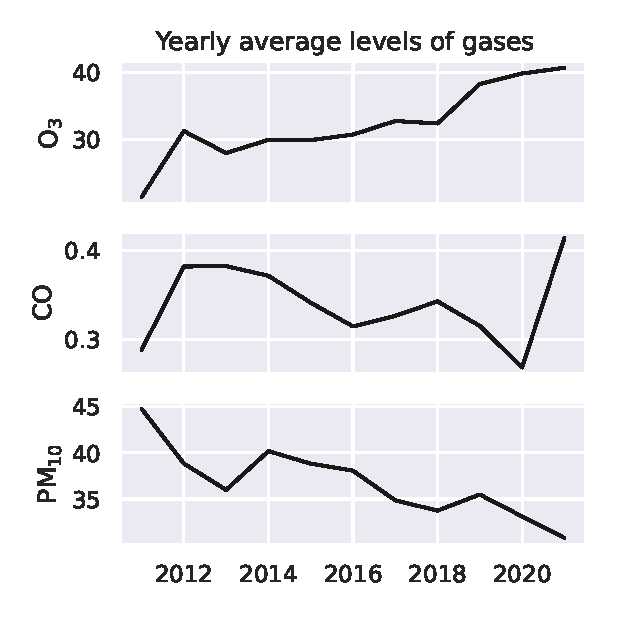
\includegraphics[width=.45\textwidth]{time-plots-gases-yearly.eps}
    \caption{Time series with yearly average levels.}
    \label{fig:time-series-gases-year}
\end{figure}

By Figure \ref{fig:histogram-obs-years}, years 2011 and 2021 have less
observation than the others. The year 2021 did not end as previously
mentioned and the year 2011 had less monitoring stations.  

\begin{figure}
    \begin{center}
        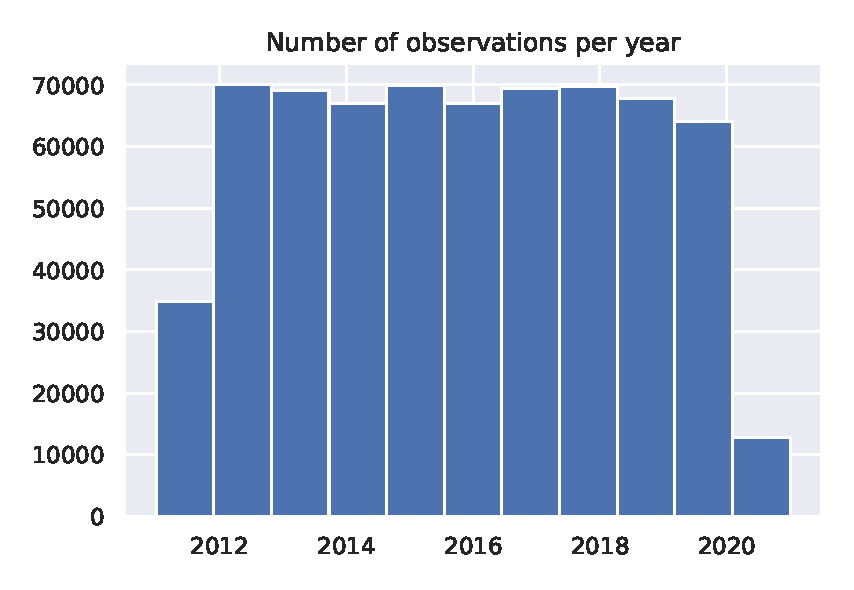
\includegraphics[width=0.47\textwidth]{histogram.eps}
    \end{center}
    \caption{Number of hourly measurements per year. In 2011, only half of the monitoring stations worked.}
    \label{fig:histogram-obs-years}
\end{figure}

Figure \ref{fig:correlation-features} shows an overview of the correlations
between different features of the data to identify possible linear relations.
The scatter plots of two to two features represents it with more details, but
there much data, and the image has a large size. It does not present anything
much different, though. The variables {\tt Temp}, {\tt UR}, and {\tt RS} are
strongly linearly related with absolute correlation greater than 0.6.

\begin{figure*}[t]
    \begin{center}
        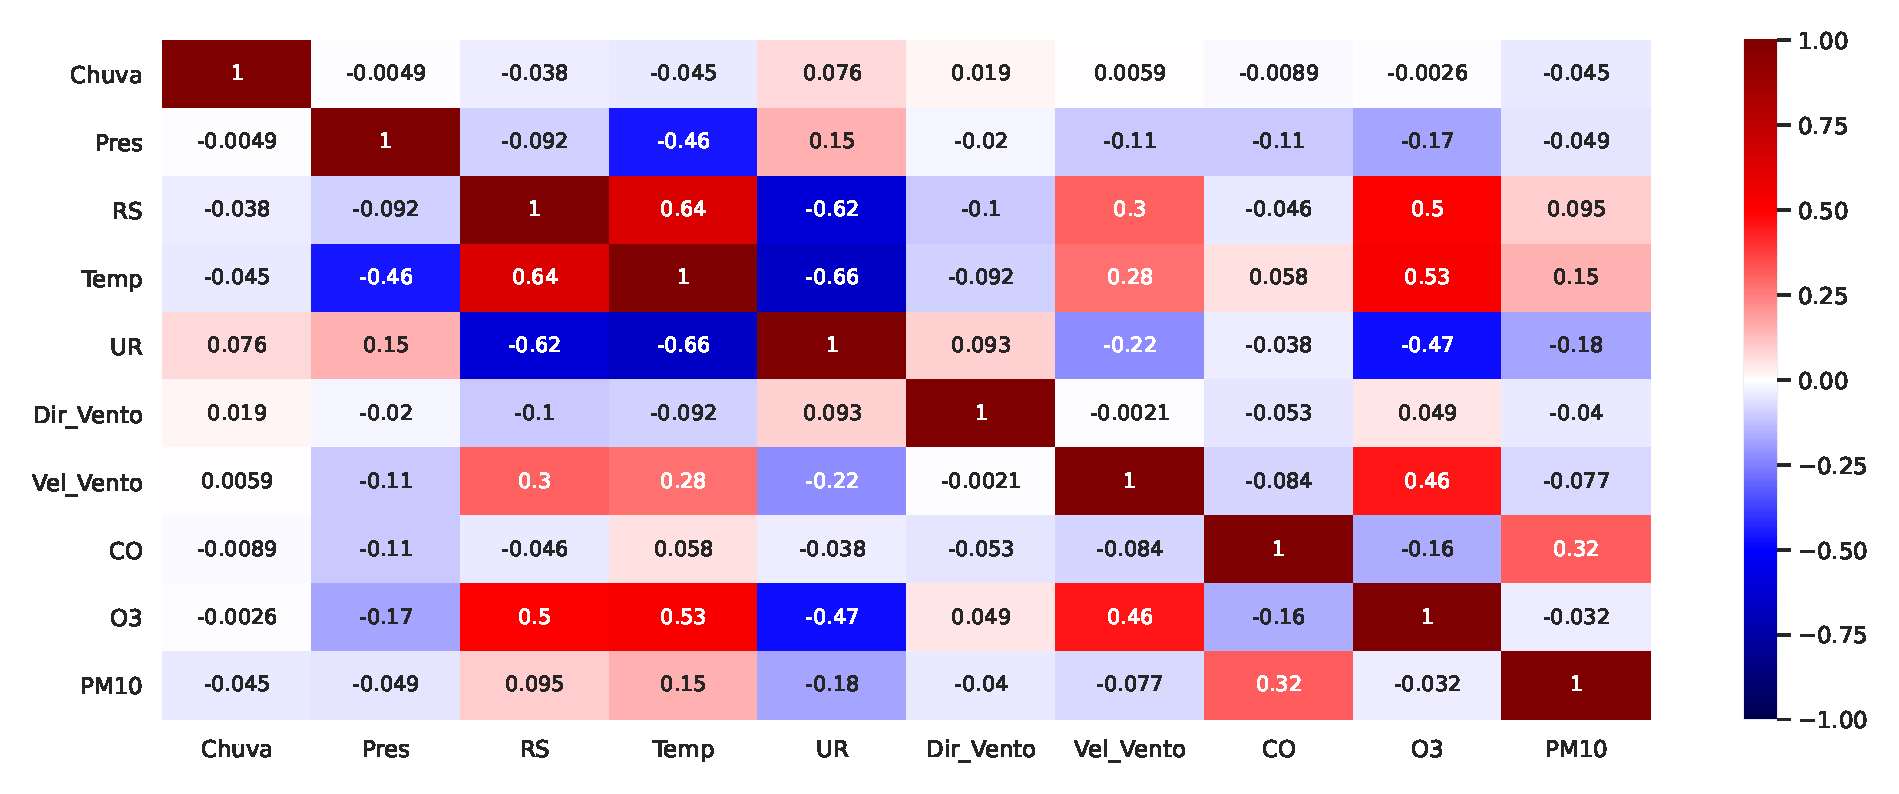
\includegraphics[width=0.9\textwidth]{correlation-graph.eps}
    \end{center}
    \caption{Correlation heat map comparing the data features.}
    \label{fig:correlation-features}
\end{figure*}

Figure \ref{fig:hourly-boxplot-ozone} shows an interesting behavior of the ozone during the day. For each hour of the day, we represent the distribution of ozone in the respective hour. We
observe that (1) the pollutants have heavy tail, or this data has a lot of
outliers; and (2) the medians go along with the movement of the sun.

\vspace{-0.5cm}

\begin{figure}[H]
    \begin{center}
        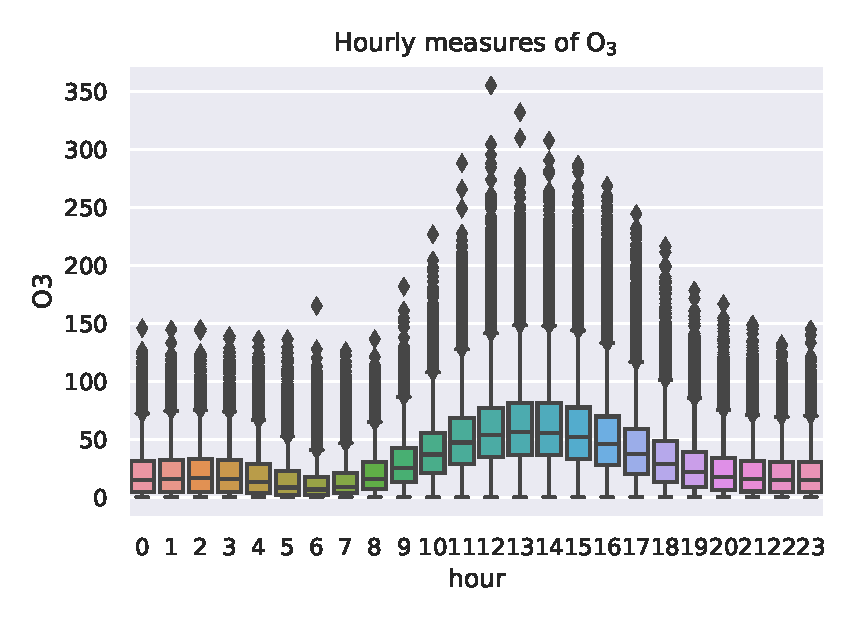
\includegraphics[width=0.42\textwidth]{hourly_measure_o3.eps}
    \end{center}
    \vspace{-0.8cm}
    \caption{Boxplot of hourly ozone measurements. }
    \label{fig:hourly-boxplot-ozone}
\end{figure}


\subsection{Data preprocessing}
\label{sec:data-preprocessing}

The data preprocessing is an important step before the usage of machine
learning algorithms, in order to report robust and neat results. Data from
year 2020 and 2021 will be removed given the pandemic in the world. 

\subsubsection{Seasonal and time features}

From the variable {\tt Data}, it is extracted the variables {\tt year, month,
day}, {\tt hour}, a boolean variable indicating the weekend, and a {\tt season} variable. In
order to consider the hourly seasonality, it is created the variables
$\text{hour\_sin} = \sin(2\pi \text{ hour}/24)$ and $\text{hour\_cos} =
\cos(2\pi \text{ hour}/24)$. 

\subsubsection{Missing data imputation}

In this dataset, there is two types of missing data: (1) monitoring stations
do not measure all pollutants by construction. For instance, it is not
measured CO in Pedra de Guaratiba; and (2) monitoring stations did not
measure in a period for some reason. For the first case, missing values remain
in the dataset and the prediction is not performed. For the second case, two
methods were compared: by location and KNN.  

\begin{enumerate}
    \item Possíveis formas de imputação: estimação polinomial de 2ª ordem.
    Alguns testes simples pode ser interessante. Para locais onde não há
    estimação, não faz sentido imputar. 
\end{enumerate}

\subsubsection{Data transformation}

We applied the Yeo-Johnson power transform \cite{yeo2000} on continuous
variables in order to approximate the data distribution to a Gaussian
distribution and to
decrease the heteroscedasticity, as suggested by \cite{gocheva2014}. In figure
\ref{fig:before-after-transform}, the gases distribution (disregarded
missing data imputation) are shown before and after the transformation. The
selected $\lambda$ for each feature was estimated through maximum likelihood.
Following the order from table \ref{tab:statistics-variables}, the values
were, approximately, 
-21.70,  11.99, -0.11, 0.28, 1.53, 0.86, -0.81, -1.58, 0.25, and 0.27. 

\begin{figure*}
    \centering
    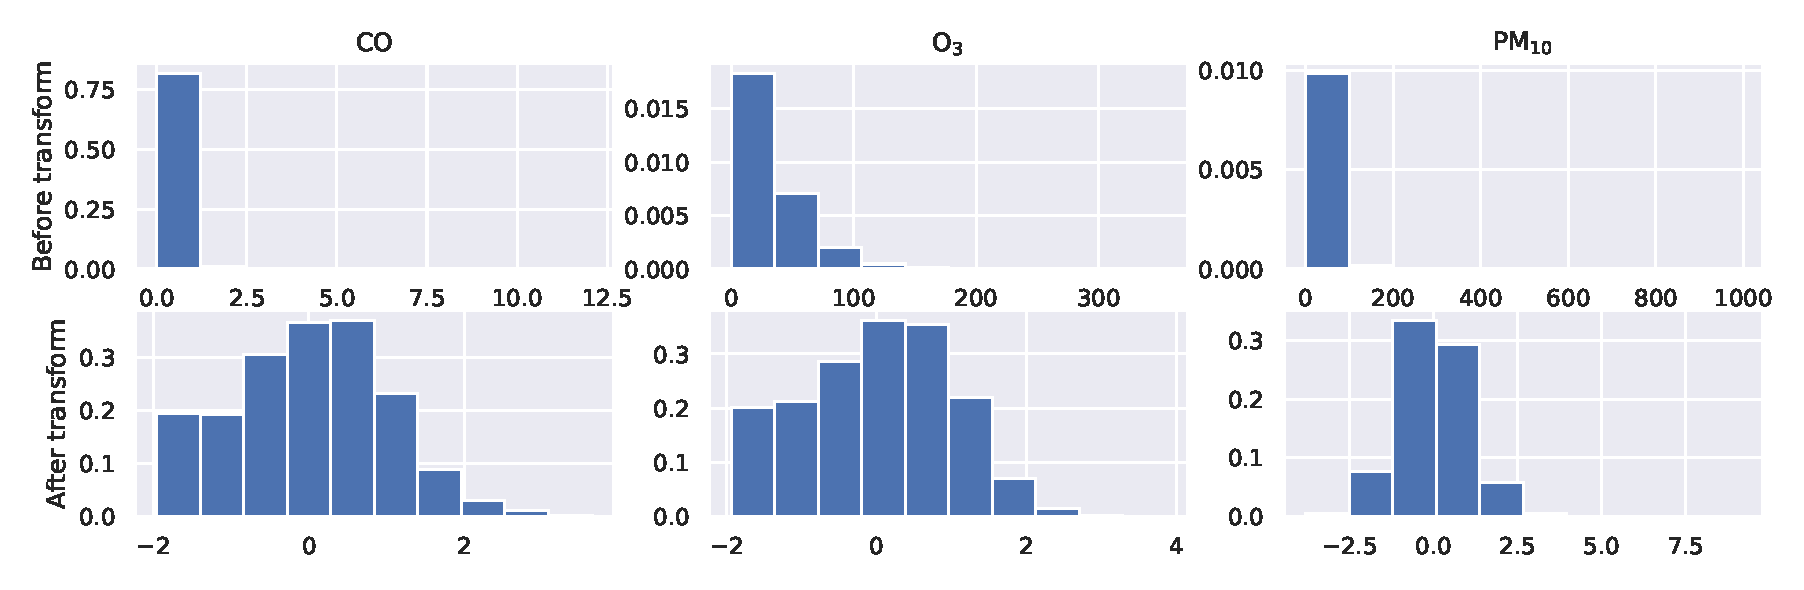
\includegraphics[width = 0.9\textwidth]{before_after_transform_gases.eps}
    \caption{Gases distribution before and after the power transform.}
    \label{fig:before-after-transform}
\end{figure*}
 
\subsubsection{Feature extraction}

\begin{enumerate}
    \item Visualize the series autocorrelation in order to define the number
    of lag variables per pollutant and particle.
    \item The number of features is XXX: lag features, roll mean features,
    weekend, season, trigonometric  
\end{enumerate}

\subsubsection{Feature selection}

Variables to remove: {\tt hour} since it is highly correlated to {\tt hour\_sin}, and {\tt Data}, because it has no service anymore. We will have
only numeric variables from now on. \com{We need to observe correlation
between lag variables from the pollutants}

\com{We applied PCA in order to reduce the dimensionality.}

